% Autor: João Fiuza de Alencastro
% Disciplina: Segurança de Redes
% Relatório 3
\documentclass[journal]{IEEEtran}
\usepackage{listings}
\usepackage[utf8]{inputenc}
\usepackage{graphicx}
\usepackage[colorlinks=true,urlcolor=red,citecolor=blue,linkcolor=blue]{hyperref}




\begin{document}

\title{Relatório Frameworks}


\author{João~Fiuza~de~Alencastro~15/0131933}% <-this % stops a space




% make the title area
\maketitle


\begin{abstract}
Relatório destinado à matéria de Segurança de Redes do Departamento de engenharia Elétrica da Universidade de Brasília. Experimento realizado enfatizando a utilização de frameworks e aplicações prontas.
\end{abstract}

\begin{IEEEkeywords}
Segurança, redes, Framework, NMap, ports, TCP, UDP, vulnerabilidade.
\end{IEEEkeywords}


\IEEEpeerreviewmaketitle



\section{Introduction}
\IEEEPARstart{R}{ealizar} experimentos utilizando ferramentas específicas, melhor desenvolvidas e de fácil acesso. Frameworks oferecem a vantagem de juntar mais de uma ferramenta de descoberta de vulnerabilidades e de testes de penetração em uma só interface. Testes de penetração são realizados de forma correta quando seguem uma sequência de ações, construindo uma base de conhecimento no início e evoluindo à medida que são realizados testes, por este motivo aplicações específicas permitem ataques mais bem estruturados. \par
Serão utilizadas algumas das ferramentas já disponíveis na distribuição do Linux Kali. Essas ferramentas, são aplicações vastamente utilizadas e são um alicerce no arsenal de ataques de \textit{'hackers'} ou \textit{'ethical hackers'}. Dentre elas estão: nmap, nikto, hydra, cisco-torch e por fim, a mais completa das aplicações, o Sparta, um framework que contempla todas as ferramentas previamente citadas.

\subsection{Aplicativos}
\subsubsection{nmap}
O conhecido aplicativo nmap deve ser realizado em etapas ou fases para ser utilizado de forma correta. Isso já é um forte indicativo que a ferramenta em questão vai muito além de um simples \textit{'port scanner'}.

%Imagem
\begin{figure}[h!]
	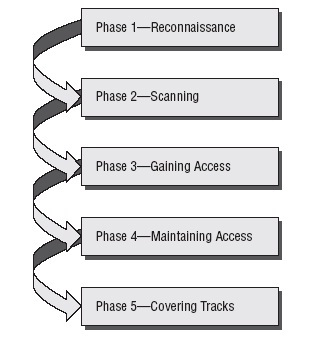
\includegraphics[width=0.65\linewidth]{../nmap_phases_pic.jpg}
	\caption{Fases de um nmap scan}
	\label{fig:nmap_phases}
\end{figure}

\subsubsection{nikto}
Baseando-se no resultado de um rápido scan no apache rodando no localhost, é visto que a ferramenta roda vários scripts de verificacão de seguranca do ambiente web. Apesar de o scan ser feito em um simples html no servidor local, o resultado é muito interessante, por mostrar o resultado de todas as verificacões. A figura abaixo mostra o resultado obtido.

%Imagem
\begin{figure}[h!]
	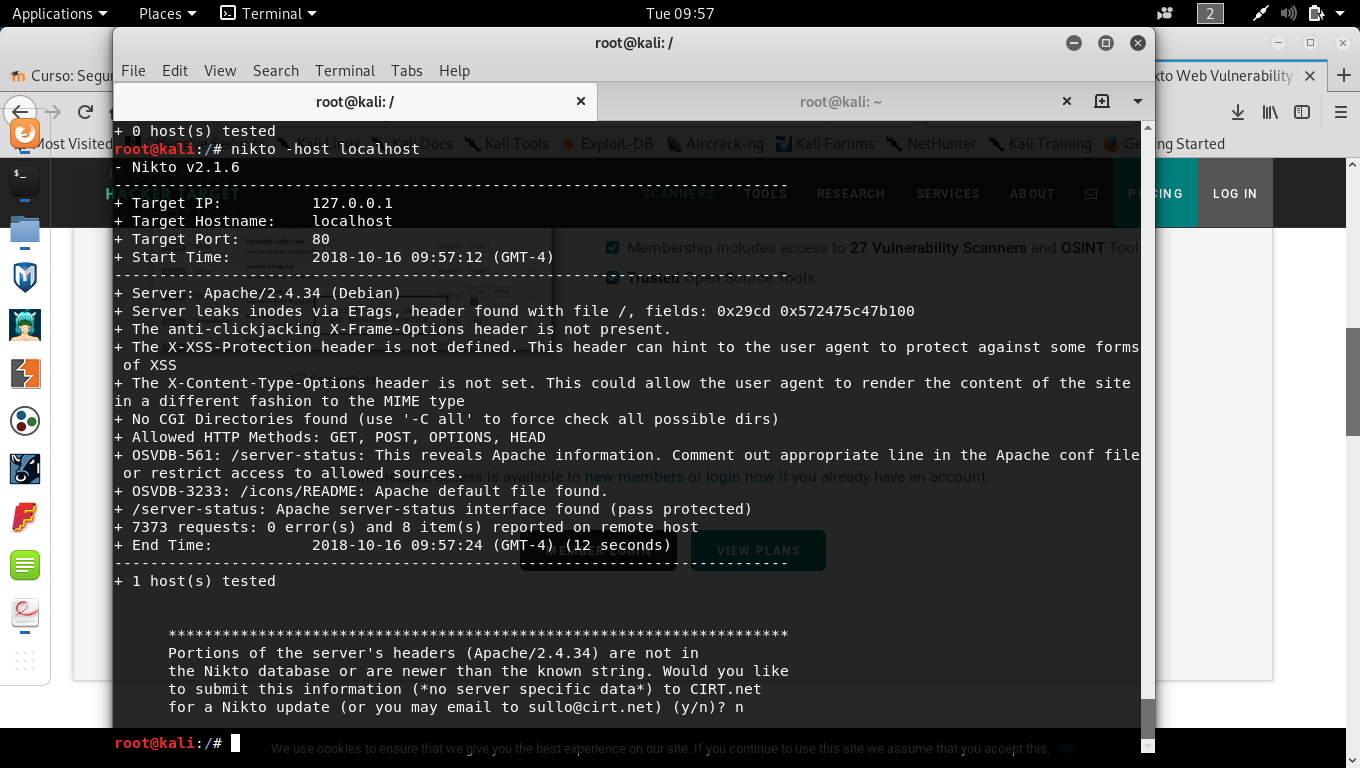
\includegraphics[width=\linewidth]{../niktoLocalhost.png}
	\caption{Resultados nikto}
	\label{fig:nikto_results}
\end{figure}

\subsubsection{hydra}
Com um resultado bem sucedido de um brute force, foi possível "quebrar" a senha de um banco de dados postgreSQL - bastante utilizado em diversas aplicações - utilizando a ferramenta Hydra. No exemplo, foi passado como parâmetro só um login, "postgres", uma lista de possíveis senhas e um host vítima do ataque. A própria ferramenta já sabe a porta padrão utilizada pelo postgreSQL, e caso a porta não fosse a padrão, a fase de pesquisa e information gathering é útil para este tipo de situação.


%Imagem
\begin{figure}[h!]
	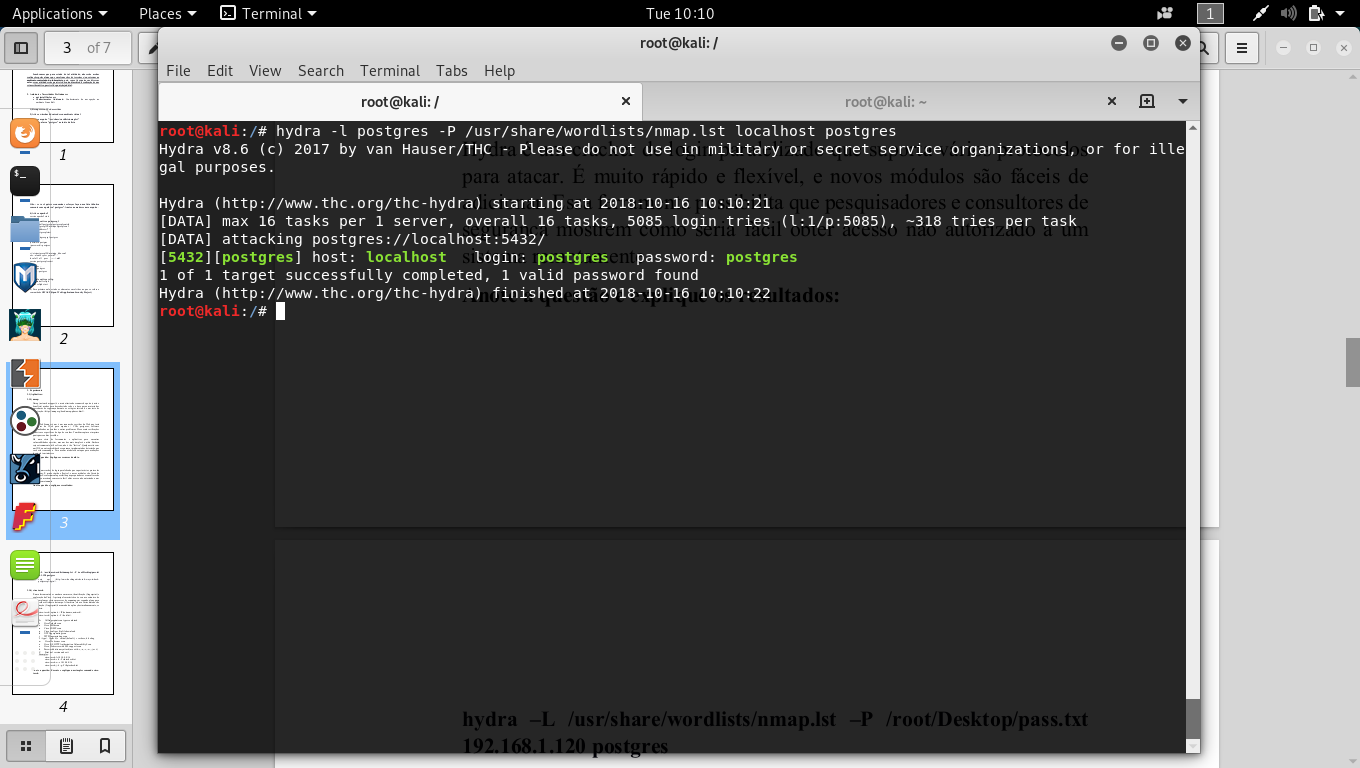
\includegraphics[width=\linewidth]{../hydraPostgresLocalhost.png}
	\caption{Resultados hydra}
	\label{fig:hydra_results}
\end{figure}

\subsubsection{cisco-torch}
Este aplicativo também é um analisador de vulnerabilidades, porém ele difere em seus métodos de análise, além de que ele distribui o processamento computacional, agilizando os procedimentos. Além disso, ele utiliza vários métodos de \textit{fingerprinting} em camada de aplicação simultaneamente. Abaixo é mostrado resultados obtidos no próprio hospedeiro local.
\\
\\
\\
\\

%Imagem
\begin{figure}[h!]
	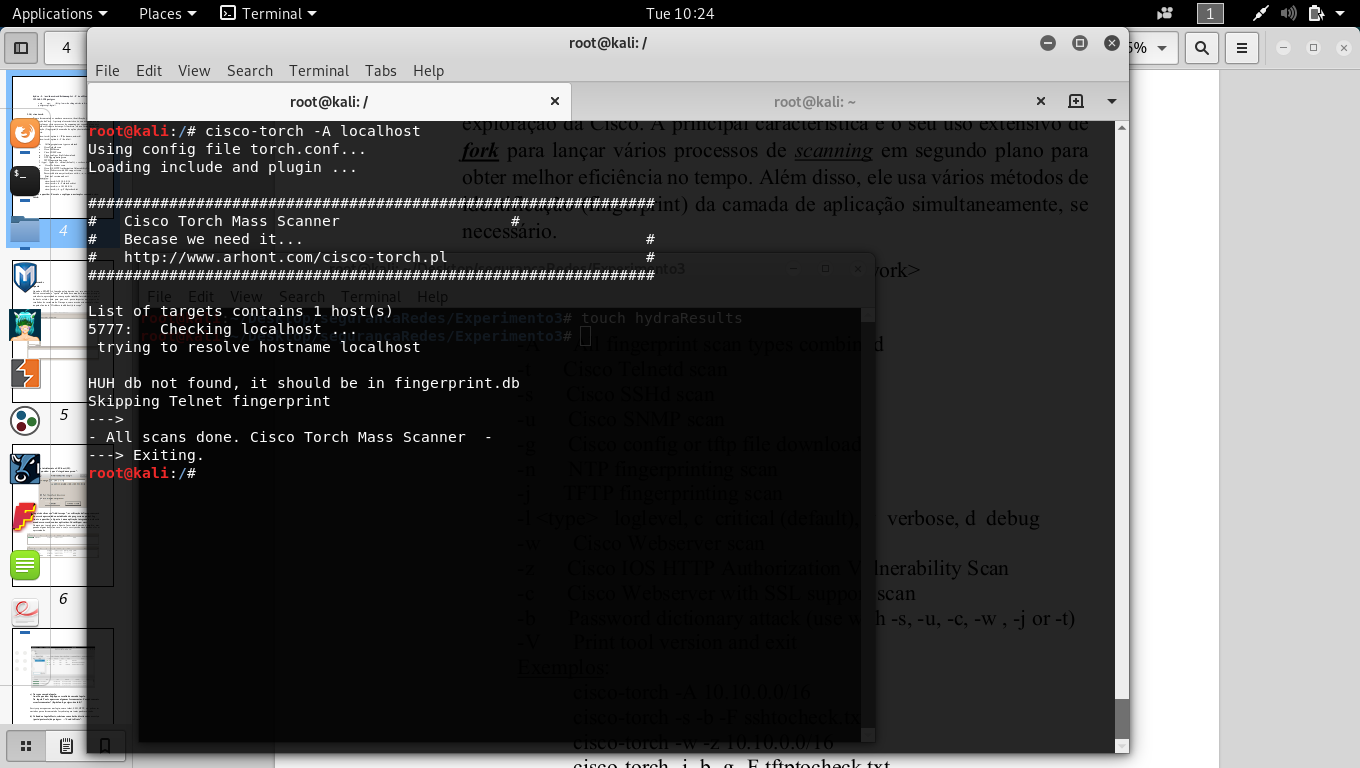
\includegraphics[width=\linewidth]{../simpleCiscoTorchLocalhost.png}
	\caption{Resultados cisco-torch}
	\label{fig:cisco_torch_results}
\end{figure}

\subsection{Frameworks}
\subsubsection{Sparta}
Os frameworks podem ser considerados a parte mais importante de um teste de penetração. Pois, eles carregam dentro de sí uma grande diversidade de ferramentas pequenas, porém extremamente úteis. Como, por exemplo, o nikto, ou o hydra. São todas ferramentas que se completam e formam um ótimo alicerce de informações sobre a vítima. \par
Antes de começar a utilizar o Sparta, foram iniciados alguns serviços comuns na máquina local, abrindo certas portas, como mostra a figura abaixo.

%Imagem
\begin{figure}[h!]
	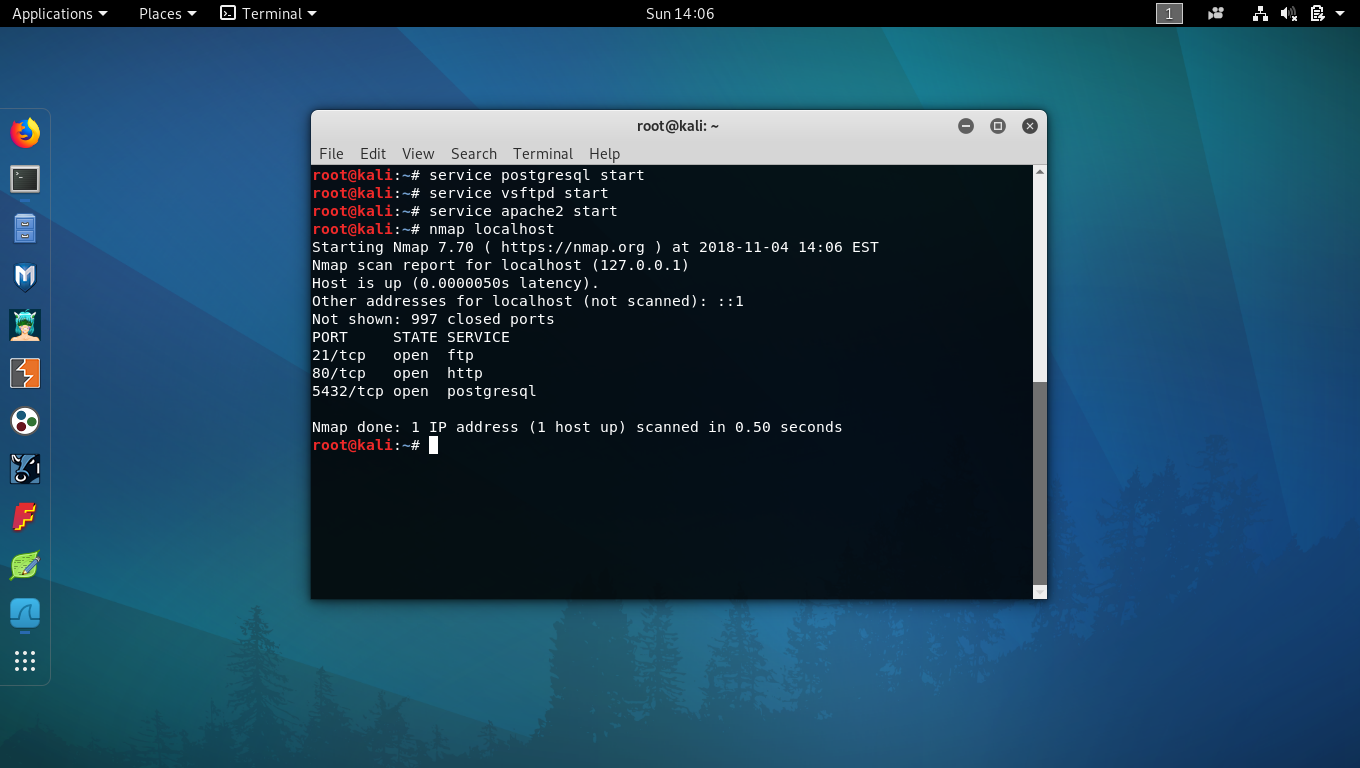
\includegraphics[width=\linewidth]{../nmap_localhost.png}
	\caption{Serviços iniciados localmente}
	\label{fig:local_services}
\end{figure}

Uma vez que os serviços estão expostos na rede, e há uma conexão estabelecida nesta mesma rede, o próprio framework se encarrega de fazer um \textit{port scan} e retorna para o usuário as portas abertas. Além disso, pode-se observar na aba de logs os scripts e tarefas que rodam no framework, como mostra a figura abaixo.
\par

%Imagem
\begin{figure}[h!]
	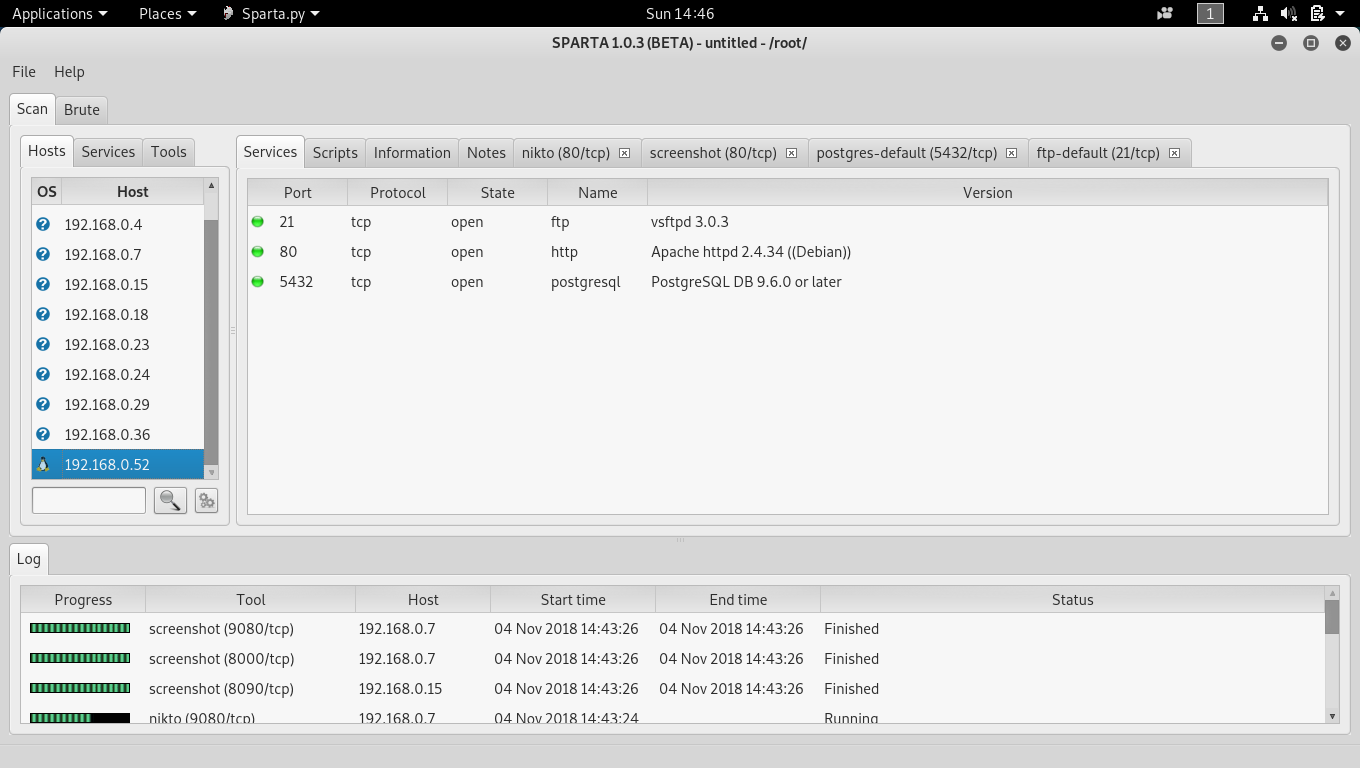
\includegraphics[width=\linewidth]{../servicos_sparta.png}
	\caption{Resultados nmap sparta}
	\label{fig:sparta_nmap_results}
\end{figure}

Depois de descobrir uma vulnerabilidade que pode ser explorada (neste caso será o postgresql), chega a hora de realizar ataques. Uma possibilidade que o Sparta oferece é o brute force da ferramenta Hydra, explicada anteriormente. Então, no próprio framework, utiliza-se o brute, apontando um nome de usuário e uma lista de possíveis senhas, como mostra a figura abaixo.
\par

%Imagem
\begin{figure}[h!]
	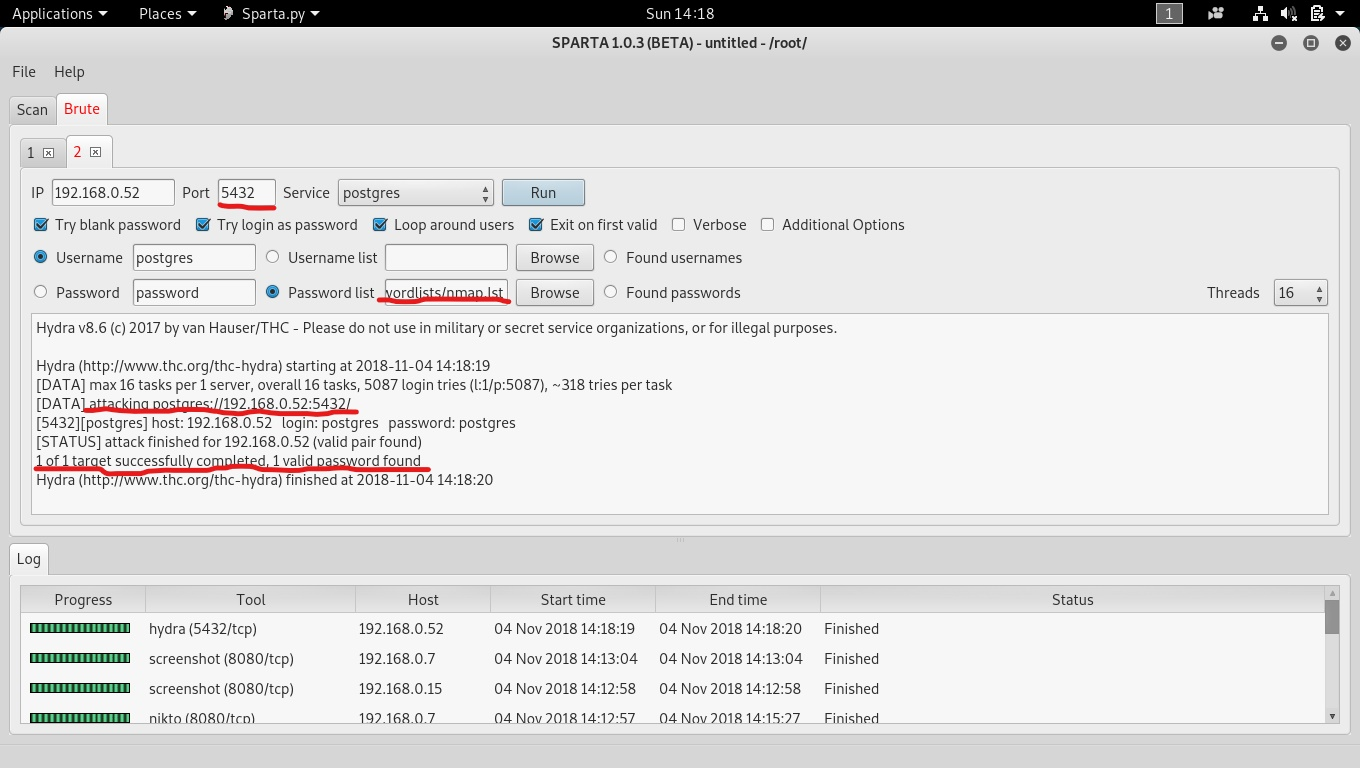
\includegraphics[width=\linewidth]{../Inkedpassword_found_brute.jpg}
	\caption{Resultado do brute force na porta 5432}
	\label{fig:brute_force_results}
\end{figure}

Foi apresentado para o usuário um ataque de força bruta bem sucedido.\par 
Agora, analisando os pacotes trafegados durante todo o experimento, pode-se observar um grande número de tentativas do framework tentando autenticar o usuário na aplicação do postgresql. A figura 8 mostra uma pequena parte do tráfego que corre "por trás dos panos". E a figura 9 mostra como é um pacote da aplicação.
\par 

%Imagem
\begin{figure}[h!]
	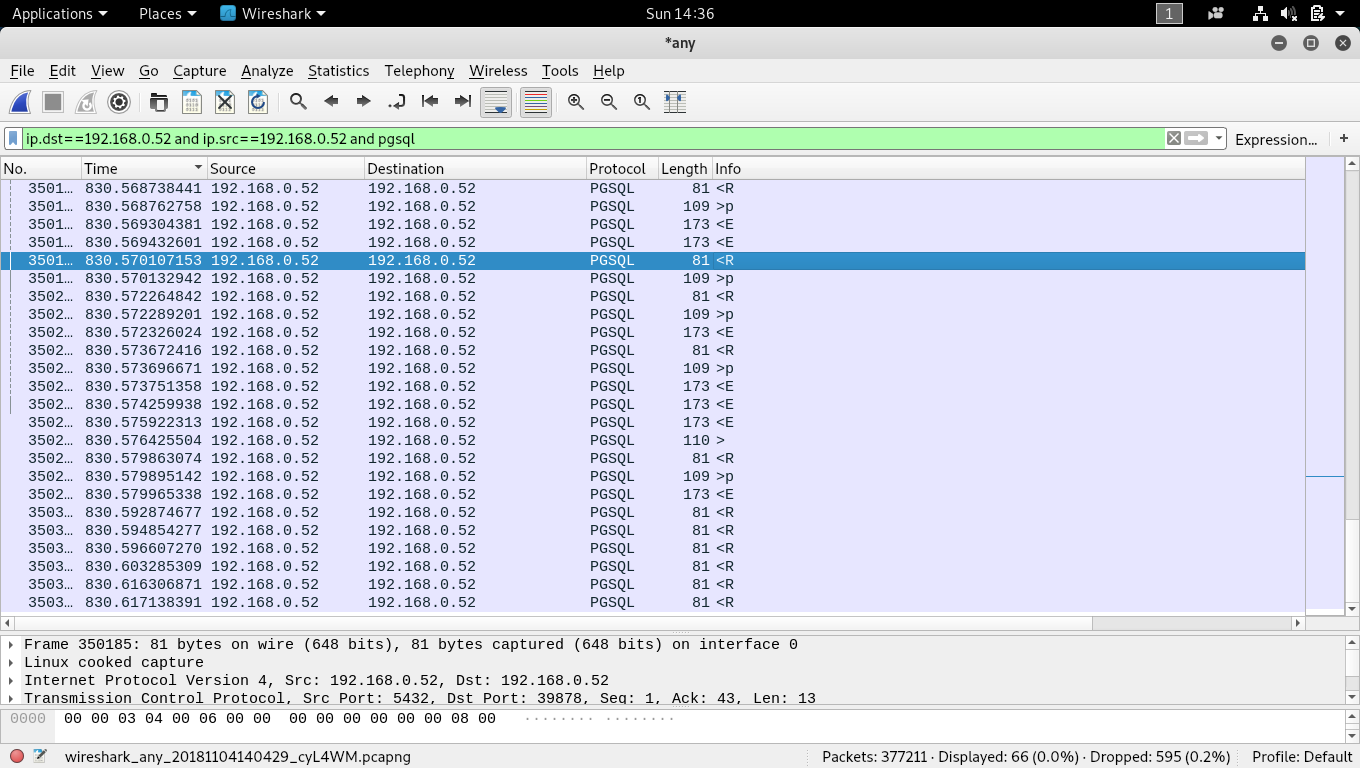
\includegraphics[width=\linewidth]{../pgsql_packets_wireshark.png}
	\caption{Pacotes da aplicação PSQL recebidos}
	\label{fig:psql_packets}
\end{figure}

%Imagem
\begin{figure}[h!]
	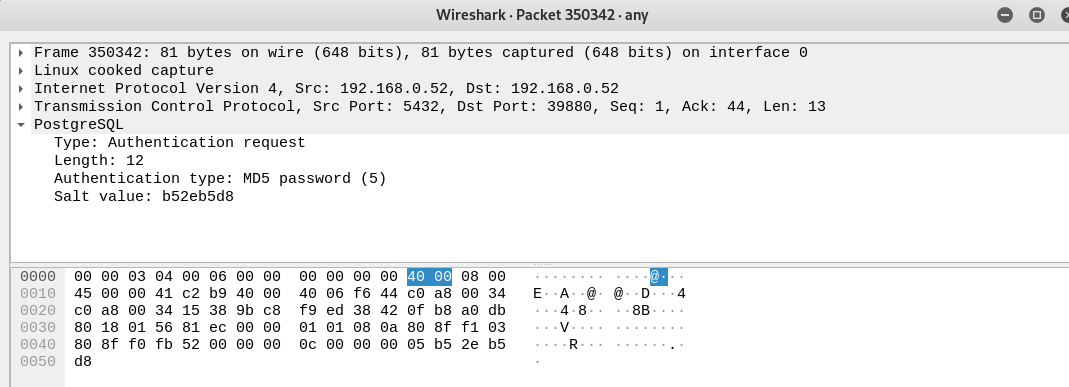
\includegraphics[width=\linewidth]{../PGSQL_application_protocol.png}
	\caption{Pacote a nível de aplicação}
	\label{fig:application_packet}
\end{figure}

Para uma análise mais profunda e cautelosa, pode-se analisar pacote por pacote, e não somente a nível de aplicação. Segundo \hyperlink{Key1}{[4]} , é possível ver o formato das mensagens trocadas por este protocolo que tem sua documentação aberta para qualquer um ler e se informar melhor, mostrando quando o pacote recebido traz uma mensagem bem sucedida ou falha.

\section{Conclusion}
A essa altura, é sabido que testes de penetração são feitos em fases, assim como a descoberta de vulnerabilidades da ferramenta nmap. Por esse motivo a utilização de aplicações e frameworks é tão útil, já que a utilização das mesmas permitem uma análise cautelosa e segmentada para um relatório bem feito. Por exemplo, se é descoberto que a aplicação vítima de ataques é uma aplicação conhecida com certas vul\-ne\-ra\-bi\-li\-da\-des, poderão ser exploradas facilmente pontos fracos específicos daquela versão daquela certa apliação. Porém, as ferramentas apresentadas neste experimento são de cunho generalizado, permitindo um estudo mais básico que dará espaço para um estudo profundo posteriormente.\par 
Foi mostrado neste experimento como um ataque pode ser custoso para o atancante também, como, o brute force, por exemplo, que precisa enviar pacotes a nível de aplicação constantemente a fim de acertar uma autenticação de um usuário. Além disso, é concluído que um ataque como o brute force pode ser facilmente evitado pela vítima se a mesma criou uma senha forte para tal aplicação, aumentando exponencialmente a complexidade do sucesso da força bruta.



\begin{thebibliography}{1}

\bibitem{cisco-torch}
https://tools.kali.org/information-gathering/cisco-torch
\bibitem{nmap-phases}
https://nmap.org/book/nmap-phases.html
\bibitem{nmap-phases-pic}
http://amaliciousmind.blogspot.com/2013/08/nmap-step-by-step.html
\bibitem{psql-message-format}
\hypertarget{Key1}{https://www.postgresql.org/docs/9.3/static/protocol-message-formats.html}


\end{thebibliography}



\end{document}


